\documentclass[12pt]{article}

% Paquetes necesarios
\usepackage[table]{xcolor} % Para colorear filas/columnas en tablas
\usepackage{graphicx}      % Para incluir imágenes
\usepackage{amsmath}       % Para ecuaciones matemáticas
\usepackage[a4paper, margin=1in]{geometry} % Configuración de página
\usepackage{tabularx}      % Para tablas con ajuste automático de ancho de columna
\usepackage{float}         % Para usar la opción [H] en tablas

\begin{document}

\begin{titlepage}
    \centering
    {\LARGE UNIVERSIDAD NACIONAL DE CÓRDOBA \par}
    \vspace{1cm}
    {\Large Facultad de Ciencias Exactas, Físicas y Naturales \par}
    \vspace{1.5cm}
    
\includegraphics[width=0.3\textwidth]{Logo-UNC.jpg} \par
    \vspace{1.5cm}
    {\LARGE \textbf{Trabajo Práctico Final - "Red de Petri / Agencia de Viajes"} \par}
    \vspace{1cm}
    {\Large \textbf{Programación Concurrente} \par}
    \vfill
    \textbf{Grupo:} \textit{Threading Bad} \par
    \vspace{0.5cm}
    - RODRIGUEZ, MATEO (43.967.398) \par
    - TRACHTA, AGUSTIN (43.271.890) \par
    \vfill
\end{titlepage}

\section{Introducción}
El presente informe detalla el trabajo realizado para abordar un problema de programación concurrente mediante el uso de redes de Petri y monitores. La programación concurrente se ha convertido en una disciplina esencial en el desarrollo de sistemas modernos, ya que permite aprovechar la capacidad de procesamiento de múltiples hilos de ejecución para mejorar la eficiencia y el rendimiento de las aplicaciones.

Sin embargo, la programación concurrente también presenta complejidades y desafíos únicos, como condiciones de carrera, bloqueos y problemas de sincronización. En este contexto, las redes de Petri emergen como una poderosa herramienta para modelar y analizar sistemas concurrentes, brindando una representación gráfica y formal de los estados y transiciones del sistema.

El objetivo principal de este informe es presentar el enfoque adoptado para resolver un problema específico de programación concurrente utilizando redes de Petri para modelar el sistema y monitores para gestionar la sincronización y el acceso seguro a los recursos compartidos. A lo largo del informe se hacen referencia a algunas definiciones que pasaremos a detallar ahora:

\section{¿Qué es una Red de Petri?}
Una Red de Petri (RdP) es un modelo matemático y gráfico utilizado para describir y analizar sistemas concurrentes y distribuidos.

\section{¿Por qué utilizamos RdP?}
Permiten modelar y visualizar casos de la vida real con paralelismo, concurrencia, sincronización e intercambio de recursos. Además, tienen un formalismo matemático y gráfico que nos permite determinar el disparo de una RdP y el siguiente marcado. Las RdP nos permiten separar la lógica de la política. La lógica es lo que puedo hacer, y la política es lo que me conviene hacer.

\section{Propiedades de la Red}
\begin{center}
    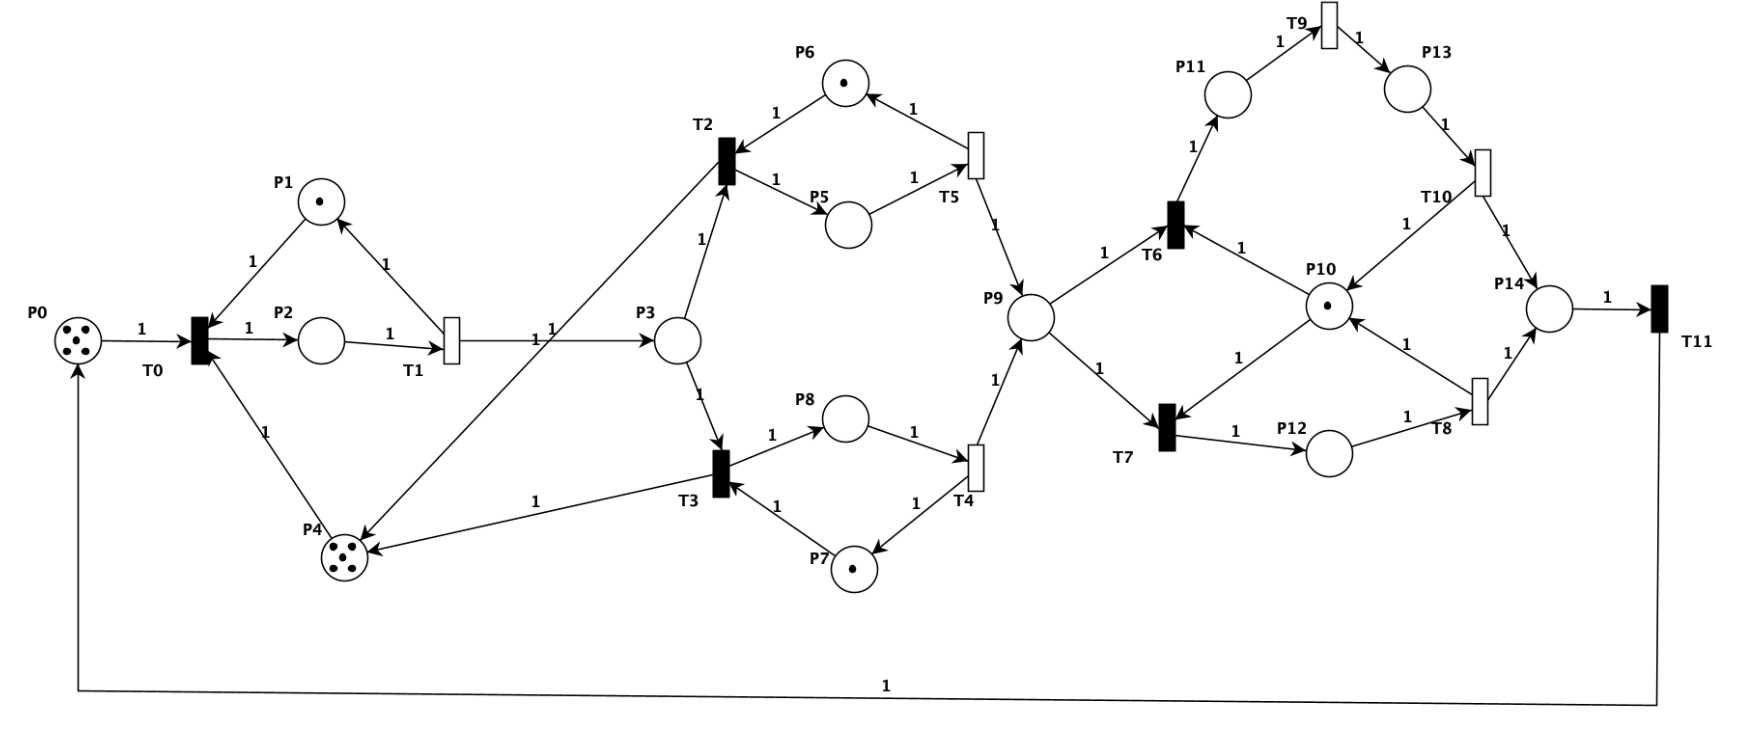
\includegraphics[width=0.9\textwidth]{Petri-Net.png}\\
    {Las siguientes propiedades a mostrar son realizadas en PIPE}
\end{center}

\begin{center}
    \textbf{Petri net state space analysis results}\\
    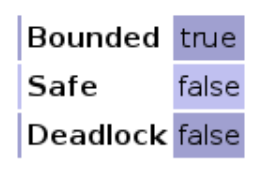
\includegraphics[width=0.4\textwidth]{Petri-Net-State.png}\\
\end{center}

\subsection{Red Limitada}
Una red de Petri es limitada si existe un límite superior para el número de tokens que puede haber en cualquier lugar de la red en cualquier momento. Esto asegura que los recursos representados por los tokens no se desborden. 
En este ejemplo, se podría decir que la cantidad de clientes que pueden ingresar y ser atendidos es limitada, por cuestiones de espacio y trabajadores.

\subsection{Red Segura}
Esta red no es segura ya que hay marcas que contienen más de un token, ya que pueden ingresar hasta 5 clientes a ser atendidos.

\subsection{Sin Deadlock}
Un Deadlock ocurre cuando un sistema queda en un estado donde no puede proceder porque todos los procesos están esperando por algún evento que nunca ocurrirá. En una red de Petri, esto significa que ninguna transición puede dispararse porque no hay tokens suficientes en los lugares necesarios para habilitar alguna transición.
En nuestro caso, al no tener Deadlock, siempre habrá al menos una transición que pueda dispararse.

\section{Invariante de Transición}
Es un vector conformado por números enteros asociados a una secuencia de disparos. Son útiles para determinar propiedades estructurales de una RdP en forma analítica. Un invariante de transición es el conjunto mínimo de transiciones que, cuando las dispare, vuelvo al estado inicial. Esto nos indica que algo se hizo. Si me fijo cuántos invariantes se completaron, voy a entender cuántos ciclos se completaron.

\begin{center}
    \textbf{Petri net invariant analysis results}\\
    \textbf{T-Invariants}\\
    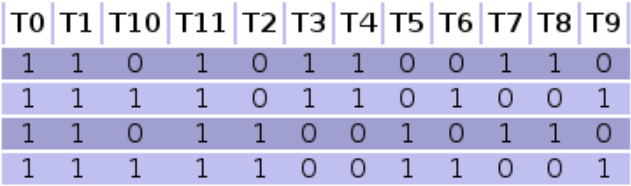
\includegraphics[width=0.8\textwidth]{T-invariants.png}\\
    \textit{The net is covered by positive T-invariants, therefore it might be bounded and live}
\end{center}

\section{Invariante de Plaza}
Un invariante de plaza es el conjunto de plazas en donde la suma de sus tokens se mantiene constante a lo largo de todos los marcados de la red.

\begin{center}
    \textbf{P-Invariants}\\
    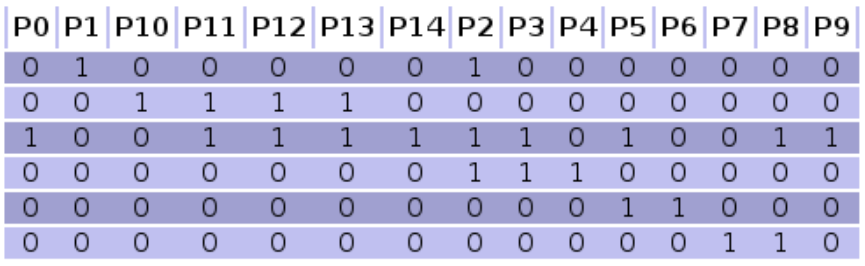
\includegraphics[width=0.8\textwidth]{P-invariants.png}\\
    \textit{The net is covered by positive T-invariants, therefore it is bounded.}
\end{center}

\subsection{Bounded and live}
El programa quiere decir que, además de estar acotada (bounded), la red siempre tiene la posibilidad de disparar alguna transición (live), por lo que no entra en un estado de bloqueo definitivo.

\subsection{Ecuaciones de Invariante de Plaza}
A continuación, se listan las ecuaciones de invariante de plaza derivadas de la red:

\[
M[P1] + M[P2] = 1
\]
\[
M[P10] + M[P11] + M[P12] + M[P13] = 1
\]
\[
M[P0] + M[P11] + M[P12] + M[P13] + M[P14] + M[P21] + M[P3] + M[P5] + M[P8] + M[P9] = 5
\]
\[
M[P2] + M[P3] + M[P4] = 5
\]
\[
M[P5] + M[P6] = 1
\]
\[
M[P7] + M[P8] = 1
\]

%---------------------------------
% NUEVA SECCIÓN: Tabla de estados
%---------------------------------
\section{Tabla de Estados en la Red de Petri}
En la siguiente tabla se detallan las plazas de la red de Petri y el estado que representan:

\begin{table}[H]
    \centering
    % Aumenta el espacio entre filas
    \renewcommand{\arraystretch}{1.2}
    \begin{tabularx}{\textwidth}{|c|X|}
    \hline
    \rowcolor{gray!20}
    \textbf{Plaza} & \textbf{Estado} \\ \hline
    P0  & Buffer de entrada de Clientes               \\ \hline
    P1  & Recursos compartidos del sistema            \\ \hline
    P2  & Cliente listo para entrar                   \\ \hline
    P3  & Cliente esperando a ser atendido            \\ \hline
    P4  & Recursos compartidos del sistema            \\ \hline
    P5  & Gestión de las Reservas                     \\ \hline
    P6  & Recursos compartidos del sistema            \\ \hline
    P7  & Gestión de las Reservas                     \\ \hline
    P8  & Recursos compartidos del sistema            \\ \hline
    P9  & Agente por cancelar la reserva              \\ \hline
    P10 & Agente por generar reserva                  \\ \hline
    P11 & Agente por confirmar reserva                \\ \hline
    P12 & Agente por pagar la reserva                 \\ \hline
    P13 & El cliente está por retirarse               \\ \hline
    P14 & (Lugar adicional según el modelo)           \\ \hline
    \end{tabularx}
    \caption{Tabla de estados en la red de Petri.}
    \label{tabla:estados-red-petri}
\end{table}

%---------------------------------
% NUEVA SECCIÓN: Tabla de eventos
%---------------------------------
\section{Tabla de Eventos en la Red de Petri}
A continuación se listan las transiciones y el evento asociado en la red de Petri:

\begin{table}[H]
    \centering
    \renewcommand{\arraystretch}{1.2}
    \begin{tabularx}{\textwidth}{|c|X|}
    \hline
    \rowcolor{green!20}
    \textbf{Transiciones} & \textbf{Evento} \\ \hline
    T0  & Input de Clientes                \\ \hline
    T1  & Cliente entra al negocio         \\ \hline
    T2  & Cliente es atendido              \\ \hline
    T3  & Cliente es atendido              \\ \hline
    T4  & Cliente pasa a la Confirmación   \\ \hline
    T5  & Cliente pasa a la Confirmación   \\ \hline
    T6  & Agente confirma la reserva       \\ \hline
    T7  & Agente rechaza la reserva        \\ \hline
    T8  & Cliente pasa a retirarse         \\ \hline
    T9  & Se paga la reserva               \\ \hline
    T10 & Cliente pasa a retirarse         \\ \hline
    T11 & Cliente se retira de la agencia  \\ \hline
    \end{tabularx}
    \caption{Tabla de eventos en la red de Petri.}
    \label{tabla:eventos-red-petri}
\end{table}


\section{Determinación de la cantidad de hilos}

Para la obtención de la cantidad máxima de hilos activos simultáneamente, utilizamos un algoritmo proporcionado por el profesor. A continuación, se detallan los resultados obtenidos:

\subsection{ Obtener los IT de la RdP}

Los invariantes de transición (IT) representan combinaciones de transiciones que pueden ejecutarse sin afectar el estado general del sistema. Se han identificado los siguientes IT:

\begin{enumerate}
    \item \{T0, T1, T3, T4, T7, T8, T11\}
    \item \{T0, T1, T3, T4, T6, T9, T10, T11\}
    \item \{T0, T1, T2, T5, T7, T8, T11\}
    \item \{T0, T1, T2, T5, T6, T9, T10, T11\}
\end{enumerate}

\subsection{ Obtener el conjunto de plazas asociadas al IT}

Cada IT está relacionado con un conjunto específico de plazas dentro de la red de Petri, lo que nos permite analizar cómo se distribuyen los recursos y estados en la concurrencia:

\begin{enumerate}
    \item \{P0, P1, P2, P3, P4, P7, P8, P9, P10, P12, P14\}
    \item \{P0, P1, P2, P3, P4, P7, P8, P9, P10, P11, P13, P14\}
    \item \{P0, P1, P2, P3, P4, P5, P6, P9, P10, P12, P14\}
    \item \{P0, P1, P2, P3, P4, P5, P6, P9, P10, P11, P13, P14\}
\end{enumerate}

\subsection{ Determinar las plazas relacionadas a acciones de cada IT}

\begin{enumerate}
    \item \{P2, P8, P12\}
    \item \{P2, P8, P11, P13\}
    \item \{P2, P5, P12\}
    \item \{P2,P5,P11, P13\}
\end{enumerate}

\subsection{  Obtenemos el conjunto de estados del conjunto de plazas PA}
\begin{enumerate}
    \item PA = \{P2, P5, P8, P11, P12, P13\}
\end{enumerate}

\subsection{ Suma de Marcas}
Valor maximo de HILOS SIMULTANEOS = 4

\section{Red de Petri final}

La red de Petri final utilizada en el programa consta de 6 segmentos.
\begin{center}
    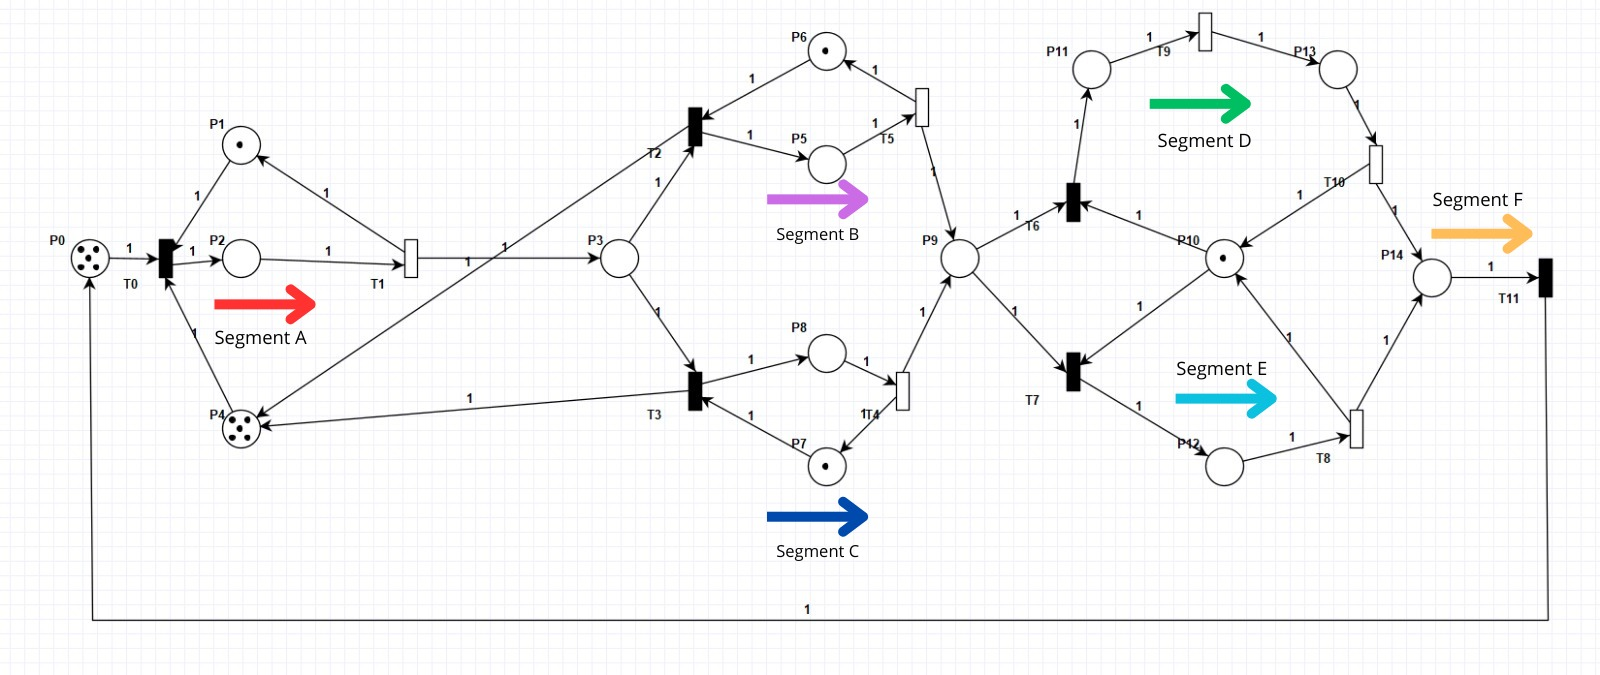
\includegraphics[width=0.9\textwidth]{Petri-Net-Final.jpeg}
\end{center}

\section{Justificación de la elección de los segmentos}

La elección de los segmentos en la red de Petri se basó en la identificación de estructuras lineales, forks y joins en la red. Cada segmento se definió con el objetivo de maximizar la concurrencia y optimizar el uso de los hilos disponibles:

\begin{enumerate}
    \item \textbf{Segmento A:} Es una secuencia de transiciones sin bifurcaciones, por lo que se ejecuta de manera secuencial sin interferencias.
    
    \item \textbf{Segmentos B, C, D, E:} Estos segmentos contienen transiciones que generan caminos en paralelo (forks). Al dividir la ejecución en hilos independientes, se evita que un solo hilo tenga que decidir qué camino seguir, delegando la decisión a la política de ejecución del sistema.
    
    \item \textbf{Segmento D:} Aunque es parte de un fork, en su parte final no comparte transiciones con otros segmentos, por lo que actúa también como un segmento lineal.
    
    \item \textbf{Segmento F:} Representa el punto de convergencia de caminos en la red (join). Para evitar bloqueos, se permite la ejecución paralela de los segmentos anteriores, asegurando que todas las dependencias se resuelvan antes de continuar con la ejecución final.
\end{enumerate}

\section{Determinación de hilos máximos por segmento}

A partir de la segmentación de la red de Petri y la identificación de los subconjuntos de plazas asociadas a cada segmento, se determina la cantidad máxima de hilos que pueden ejecutarse simultáneamente. La segmentación permite dividir la ejecución en partes independientes, asegurando que no haya interferencias en la ejecución concurrente.

Cada segmento tiene un conjunto de plazas asociadas, denominadas \(PS_i\), que representan los estados alcanzables en dicho segmento. A continuación, se presentan los segmentos con sus respectivas plazas y la cantidad máxima de hilos necesarios para su ejecución:

\begin{itemize}
    \item \(PS_a = \{P2\} \Rightarrow \text{MAX} = 1\)
    \item \(PS_b = \{P5\} \Rightarrow \text{MAX} = 1\)
    \item \(PS_c = \{P8\} \Rightarrow \text{MAX} = 1\)
    \item \(PS_d = \{P11, P13\} \Rightarrow \text{MAX} = 1\)
    \item \(PS_e = \{P12\} \Rightarrow \text{MAX} = 1\)
    \item \(PS_f = \{P14\} \Rightarrow \text{MAX} = 1\)
\end{itemize}

Dado que cada segmento requiere un hilo para su ejecución, la suma de los hilos necesarios en todos los segmentos nos da la cantidad total de hilos que el sistema puede necesitar en toda su ejecución:

\[
Hilos\ totales\ del\ sistema = 1 + 1 + 1 + 1 + 1 + 1 = 6
\]

Sin embargo, esto no significa que en todo momento haya 6 hilos ejecutándose en simultáneo.  
El primer algoritmo determinó que la **máxima cantidad de hilos activos simultáneamente** en la red de Petri es **4**, lo que significa que en el punto de mayor concurrencia del sistema, pueden llegar a ejecutarse hasta 4 hilos a la vez.  
La segmentación realizada permite distribuir la carga de trabajo de manera eficiente, asegurando que cada hilo ejecute su parte sin interferencias y maximizando el rendimiento del sistema.

\end{document}
